% Font size needs to be at least 12-pt.

\documentclass[12pt]{article}
\usepackage[utf8]{inputenc}
\usepackage{amsmath}
\usepackage{amssymb}
%\usepackage[left=1.0in,right=1.0in,top=1.0in,bottom=1.0in,pdftex]{geometry}
\usepackage{fancyhdr}
\usepackage{setspace}
\usepackage{lastpage}
\usepackage{graphicx}
\usepackage[style=numeric]{biblatex}
\addbibresource{bibliography.bib}
\usepackage{comment}

\fancypagestyle{firststyle}
{
   \fancyhf{}
   \lhead{\textbf{Problem Chosen}\\ \Large{\textbf{Problem A}}}
   \chead{\textbf{2020}\\ \textbf{MCM/ICM}\\ \textbf{Summary Sheet}}
   \rhead{\textbf{Team Control Number}\\ \Large{\textbf{2018285}}}
   %\cfoot{\thepage}
   %\topmargin -0.5in
   \setlength{\headheight}{44pt}
   %\setlength{\footskip}{20pt}
   \renewcommand{\headrulewidth}{2pt}
}

\pagestyle{fancy}
\fancyhf{}
\rhead{Control\# 2018285} 
\lhead{Page \thepage\ of \pageref{LastPage}}
\cfoot{\thepage}
%\setlength{\headheight}{20pt}

\title{Where Are The Fish?}
\author{Control\# 2018285}
\date{February 17, 2020}

\begin{document}

\thispagestyle{firststyle}

With global ocean temperatures on the rise, fish populations are moving into different habitats in order to survive. This has fishing businesses concerned with how to keep their businesses running. In particular, changes in the Scottish herring and mackerel populations have smaller Scottish fishing companies concerned with how to feasibly operate under these changing conditions.

Using available data, we have constructed an advection model to estimate where Scottish herring and mackerel populations will be within 50 years. For each species, we examine two main locations: the western Scottish coast and the eastern Scottish coast. Specifically, we determined possible speeds at which each population will migrate north, and used that to predict how the population distribution will change over time. We determined speed parameters using a number of factors including the rate at which the water temperatures surrounding the island would increase as well as the different habitable temperature ranges for herring and mackerel. 

We assume that if the water temperatures pass maximum threshold levels for fish habitats, then most of the fish populations would migrate out. We examine best, average, and worst case scenarios for these thresholds.

In our analysis, we focused on the 57 degree latitude marker on the island as that was the upper end of the Scottish territory and we looked at what percentage of the fish population remained below that marker after a time span of 50 years. The latitude interval from 57 degrees and above represents the last possible locations where fisheries could base their operations out of before the populations fully departed from the of the island. 

We recommend that fishing companies focus less on fishing for herring and more on fishing for mackerel, as our model projects mackerel leaving the island and surrounding waters far less quickly than herring. As for possible domestic relocation, we recommend that fishing companies relocate their operations closer to the northeastern coast of Scotland.


\newpage 

\setcounter{page}{1}
\maketitle

%\begin{abstract}
%    Abstract goes here.
%\end{abstract}

\newpage
\tableofcontents
\newpage

\section{Introduction}
Fishing is one of the essential keys to the Scottish economy. Besides being a popular hobby, it is also considered as an important role for Scottish marine industrial development and a way of life for both rural and urban communities in Scotland \cite{marine_economy}. Inside Scottish marine industrial development, some of the top marine species such as mackerel and herring have greatly contributed to the value of landings for Scottish vessels between 2017 and 2018 \cite{scot_fishery}. However, based on the table from this source \cite{scot_fishery}, the value of landings of both mackerel and herring were not as high as the other species. For this reason, we see that external factors such as rising water temperatures will cause the fish population to migrate to the north (where the water temperatures are lower). Our goal is to take existing temperature data for the Scottish shores and form a model which will help us predict the migration of Scottish mackerel and herring stocks. Further, based on our model's predictions, we give recommendations for Scottish fishery management companies to make appropriate changes in their operations.

\section{Assumptions}

\begin{enumerate}
    \item \textbf{Northward movement.} Recent research suggests that in response to global increase in sea temperatures, many fish populations are moving away from the equator and toward the poles \cite{findlay_2020, gigy_smalls}. We assume that the mackerel and herring populations surrounding Scotland and neighboring territories exhibit this same behavior. According to research made by Cindi \cite{Cindi}, fish prefer to sustain in cold water because they do not have to breathe as fast due to their metabolism being slowed down which does not require much oxygen. Moreover, this article \cite{Cindi} showed that cold water contains more dissolved oxygen than warm water so that the fish do not have to work as hard in order to extract the oxygen. 
    \item \textbf{Uniform rate of temperature change.} We assume that at any given time, the water temperature in all sea areas is rising at the same rate. We believe this is true based on what Borunda \cite{borunda} stated about the global temperature from the Nation Geographic, we human being have burned massive amount of fossil fuels since the beginning of the Industrial Revolution, exploited a huge number of forests, and undertaken many other activities which causes carbon dioxide emission. Due to these factors, they have led to the problem which we know over periods of time to be "Global Warming" which included ocean warming. 
    
    \item \textbf{Straight on each side of Scotland.} We treat the west and east coasts of Scotland as running straight, north and south. This is far easier to use in a model than a nonlinear, irregular shoreline. Additionally, this assumption allows us to more easily predict how far north the herring and mackerel populations will move, as there is effectively only one dimension of movement to consider in this simplification.
    
\begin{figure}[h]
\begin{center}
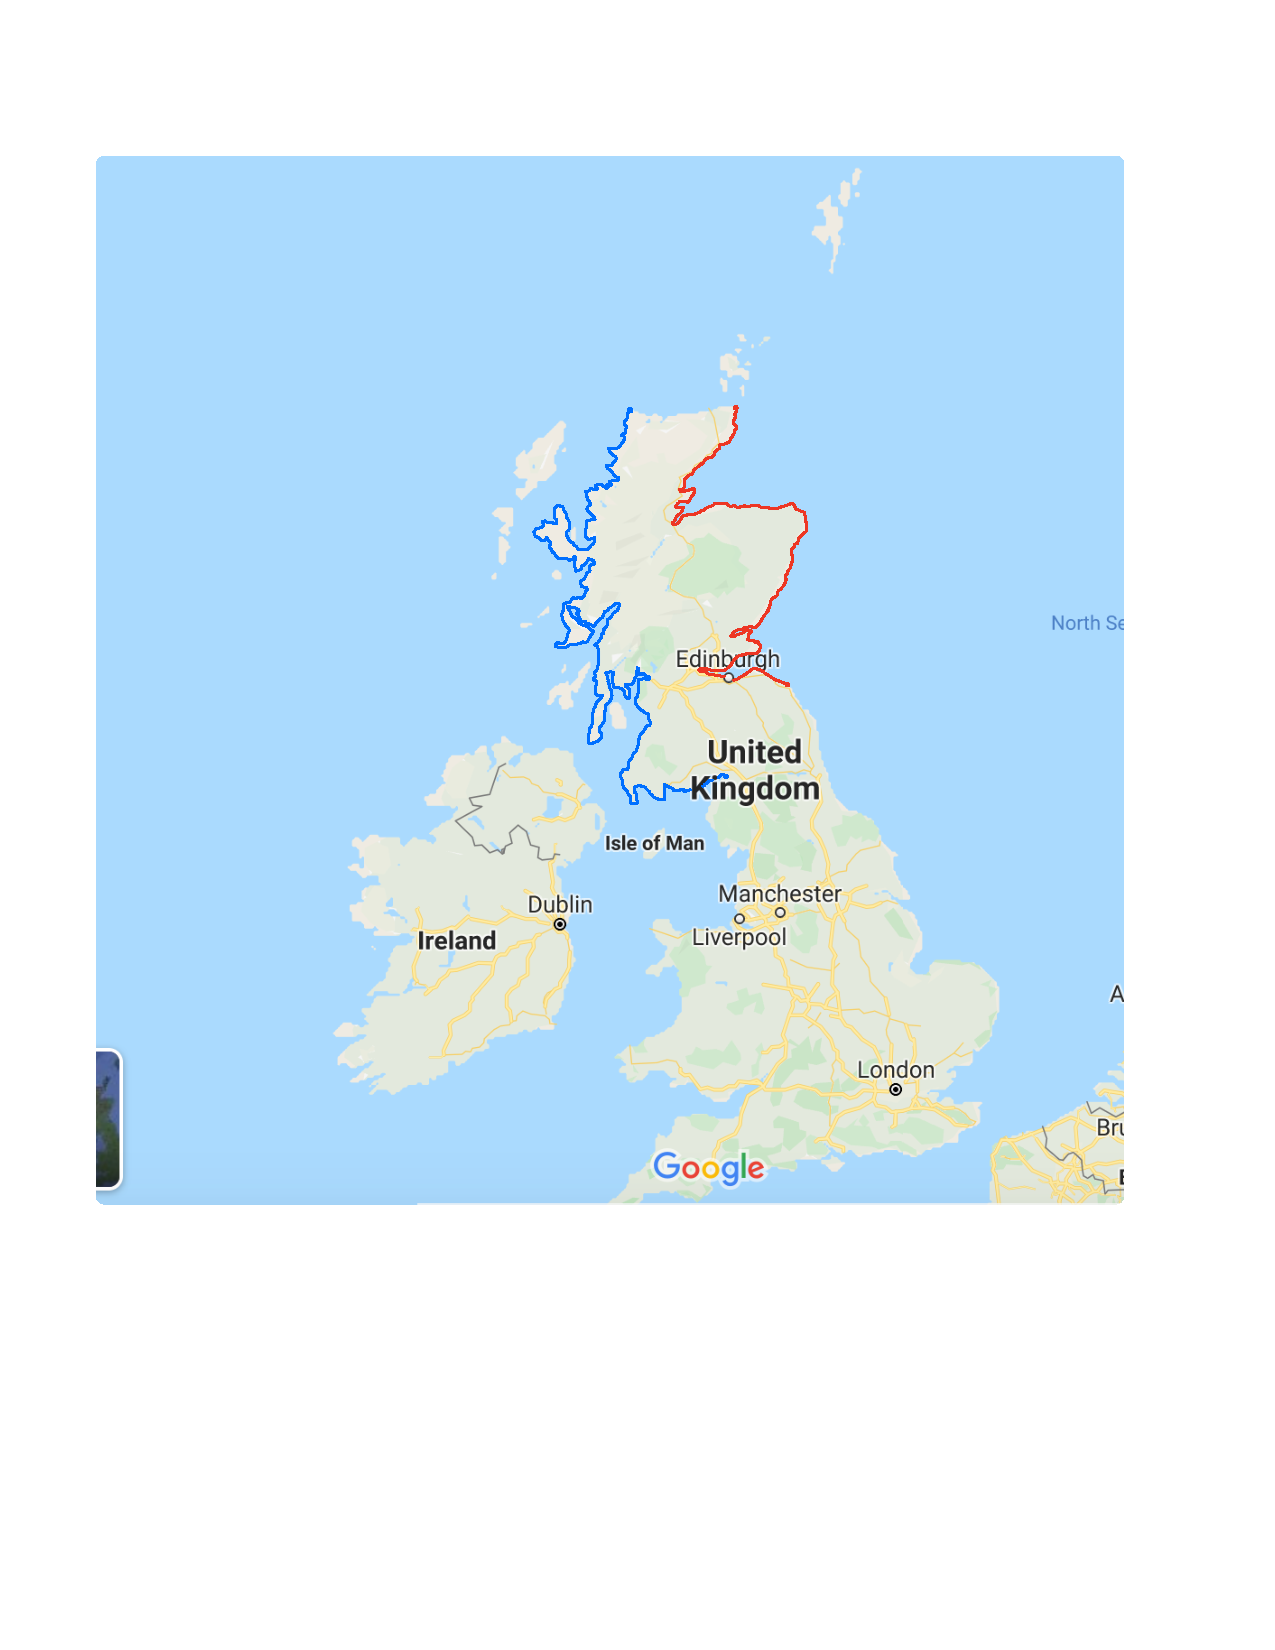
\includegraphics[width=13cm]{Scot_Map.pdf}
\caption{Map of Scotland, blue line is the Western domain, red the Eastern \cite{uk_map}.}
\end{center}
\end{figure}

    \item We are assuming that the Spawning Stock Biomass (SSB) is an effective population measure for us to use in our model. We believe this to be a relevant and effective assumption because the International Council for the Exploration of the Sea (ICES) gives its recommendations for stock management using this measure.
\end{enumerate}

\section{The Model}

Our model is based on the advection equation, a partial differential equation (PDE) that models the bulk transport of some material in a fluid medium. In this case our medium is the Atlantic ocean surrounding the island of Scotland, and the material being advected is both the mackerel and herring fish species. The one dimensional advection equation is 
$$\frac{\partial u}{\partial t}= -c \frac{\partial u}{\partial x}$$
A solution to this equation is of the form $u(x,t) = f(x-ct)$ where the function is arbitrary and differentiable with respect to both time and space. 
Specifically, our solution to this model is
\[
u(x,t) = e^{-r(x-ct)^2}
\]
where 
\begin{itemize}
    \item \(u(x,t) = \) the population density.
    \item \(r = \) the density parameter.
    \item \(x = \) the latitude of a region.
    \item \(t = \) the time.
    \item \(c = \) the advection speed.
\end{itemize}

Our model assumes that the direction of the flow of these species will be northward toward colder waters. We think this is a reasonable assumption as much of the literature we found predicts this sort of movement for most fish species \cite{findlay_2020, gigy_smalls}. 
Since we are trying to determine where the fish are most likely migrating to, we believe that our model will be able to predict how quickly the fish populations will relocate out of the certain fishing towns based on a number of factors including the rate at which the average global temperature is increasing, as well as the maximum temperature that the fish can live in.

\subsection{Parameters}
When it comes to determining our $c$ parameter for the speed of migration, we know that it will be influenced by a number of factors. The first is temperature change. For this we assume that our domains of Eastern and Western Scotland will have a uniform growth rate in temperature and a uniform initial temperature. We think both of these assumptions are fair due to the data that we collected \cite{tempData}. After averaging the average monthly temperatures for the past ten years at different latitudes, our data [Fig 1, Fig 2] shows uniform temperatures at $10^{\circ}$ C all along our domains. 

\begin{figure}[h!]
\begin{center}
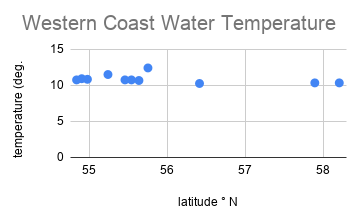
\includegraphics[width=11.5cm]{West_Coast.png}
\caption{Western Coast Water Temperature vs. Latitude.}
\end{center}
\end{figure}

\begin{figure}[h!]
\begin{center}
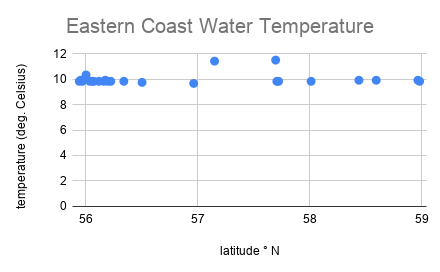
\includegraphics[width=12cm]{East_Coast.png}
\caption{Eastern Coast Water Temperature vs. Latitude.}
\end{center}
\end{figure}

For our temperature growth rate model, we assume its of exponential form, although the growth rate we choose from the literature \cite{waterTemp} is extremely modest:

$$f(x) = e^{0.013x}+10$$

where \textbf{0.013} is the change in water temperature per year \cite{waterTemp}, \textbf{10} is the initial temperature in degrees Celsius, and \textbf{x} is the time it takes to reach a certain temperature threshold.

We use this model to predict the time after which the majority of the fish species will have migrated out of the Scottish domains. To do this, we use the maximum temperatures that the fish species can live in, and we assume that when the temperatures exceed these thresholds, the fish populations will have left already \cite{gigy_smalls}. Our best, worst, and average case scenarios are dictated by the upper, lower, and average maximum temperatures in which the fish can live.

We let $M_{\textbf{thresh}}$ and $H_{\textbf{thresh}}$ denote mackerel and herring temperature thresholds respectively. For our best, average, and worst case scenarios respectively, we have $M_{\textbf{thresh}}=27,22.5,17,$ and $H_{\textbf{thresh}}=25,17.5,13$ \cite{ICES_mackerel, herr_SSB}. 
We use these numbers to approximate the time at which the fish will migrate out of the given domain. For instance, we see that $f(155) \approx 17.5 = H_{\textbf{thresh}}$, and $f(199) \approx 22.61 = M_{\textbf{thresh}}$.\\\\
We denote $T_H$ and $T_M$ as the times after which the herring and the mackerel will have mostly migrated out. Hence, for our average case scenario we have
$T_H=155$ and $T_M= 199$ years.
We now have all the parts to calculate the speed coefficient for our advection equation, where $c= \frac{\textbf{length of domain}}{\textbf{time of species migration}}$, where length of domain will be expressed in degrees latitude, and time of species migration will be in years. (We will explain what $\gamma$ is shortly.)

For each $c$, if $T$ is the threshold value, then:
\[c = \frac{(\gamma + 58.643099) - 55.810478}{T} \qquad \text{for eastern populations},\]
\[c = \frac{(\gamma + 58.625849) - 55.810478}{T} \qquad \text{for western populations}.\]

In the average case scenario:
\begin{align*}
    c_{\textrm{eastern herring}} &= 0.021066465 \\
    c_{\textrm{western herring}} &= 0.02643 \\
    c_{\textrm{eastern mackerel}} &= 0.016407 \\
    c_{\textrm{western mackerel}} &= 0.0205849 
\end{align*}

Best case scenario:
\begin{align*}
    c_{\textrm{eastern herring}} &=  0.0156737\\
    c_{\textrm{western herring}} &= 0.0155909 \\
    c_{\textrm{eastern mackerel}} &= 0.0149814 \\
    c_{\textrm{western mackerel}} &= 0.014902
\end{align*}

Worst case scenario:
\begin{align*}
    c_{\textrm{eastern herring}} &=  0.0384311\\
    c_{\textrm{western herring}} &=  0.0386352\\
    c_{\textrm{eastern mackerel}} &=  0.0217090\\
    c_{\textrm{western mackerel}} &= 0.0218243
\end{align*}

In these calculations, we let \textbf{\(\gamma\)} be the extra distance traveled out from our domain (top notch and bottom notch of the shore). In other words, \textbf{\(\gamma\)} represents how far out approximately a boat can travel in one day. From the search results given by Google, we assumed that a small fishing boat can go out within 30 miles (48 km). Since our domain represents the latitude, we then convert \textbf{\(\gamma\)} to latitude, so $\gamma=0.4324$ degrees latitude. Given that we have the latitude for the \textbf{\(\gamma\)}, we started our first calculation by finding the total length of the island which fish can travel. To find out how long it takes for fish to move from bottom to top notch of the island, we used our temperature growth rate above to determine the total time it takes for both mackerel and herring to migrate to north. When we found the value of \textbf{x} (time it takes to reach temperature threshold), we estimated that it would take \textbf{199 years} for the mackerel and \textbf{155 years} for the herring to migrate to north away once the water temperature reached certain thresholds for both.

\section{Results and Interpretation}
\subsection{Where will the fish be in the next 50 years?}

The following results were gained by integrating our normalized function $u(x,50)$ from the bottom our domain to the 57 degrees latitude mark. Those numbers corresponded to the remaining fish within that domain. We set the time variable to 50 as we wanted to see where the distribution of fish was after 50 years. For each of the cases we varied our c parameter for the necessary value.

\subsection{Average Case}
This assumes that the fish will migrate at medium speeds for 50 years. For herring on the eastern side $53\%$, will have remained within the latitude 57 degrees by 50 years. For the mackerel, $66\%$ will have remained.

For the western domain, only $37\%$ of the herring will have remained within that latitude mark. For the mackerel, $54\%$ will have remained.

\subsection{Best case}
This assumes that the fish will migrate at the slowest speeds for 50 years. On the eastern domain, $69\%$ of the herring will have remained within the 57 degrees latitude. For the mackerel, $70\%$ will have remained,

On the western domain, $69\%$ of herring will have remained within the 57 degrees, and $71\%$ of the mackerel.  

\subsection{Worst case}
This assumes that the fish will migrate at the fastest speeds. On the eastern domain, only $11\%$ of the herring will have remained within the 57 degrees mark. On the other hand $50\%$ of the mackerel will have remained within that mark.

On the western domain, we found similar results to the eastern domain with $11\%$ of the herring remaining and $50\%$ of the mackerel remaining.

\subsection{Recommendations}
Based on these results we believe that the best options for small scale fishing companies would be to fish for more mackerel as their populations will not migrate away as quickly as the herring. We see this in the data as in the average case, $66\%$ of the mackerel remained on the eastern domain while only $53\%$ of the herring remained. 

In terms of location, we recommend holding off from building any long term equipment and facilities on the western domain as the fish appear to migrate off of that side significantly faster than eastern side. As a long term strategy, we recommend moving all equipment to the Northeastern side of the Island where the last of the fish populations will be after 50 years.

\subsection{What if the fish move into non-Scottish territorial waters?}
Unfortunately, our model as it stands does not give much useful insight as to whether it would be economically attractive for fishing companies to move their bases of operations beyond domestic (Scottish) ports. 


\section{Strengths And Weaknesses of The Model}
Our model is greatly simplified compared to existing models used by researchers and organizations to predict and model population dynamics. Hence, although it is easy to construct our models and interpret its results, there are still several important missing factors:

\textbf{Strengths:} 
\begin{itemize}
    \item Our model gives us an estimate of amount of time that it takes for the fish to migrate.
    \item Our model considers the temperature in different regions.
    \item Our model gives us an estimate of how fast the fish can move.
\end{itemize}

\textbf{Weaknesses:}
\begin{itemize}
    \item Our model does not consider the longitude of regions in the north.
    \item Our model does not consider the distribution of fish population in the north.
\end{itemize}

\section{Model Improvements}

With the strengths and weaknesses of the model we have, there are definitely ways that we can modify our model so that it can take into consideration of other main factors such as the distribution of fish population in the north. As we stated above, we designed our model to be simple enough so that we could have a fundamental understanding of the behavior of both fish species. However, another important factor that can be contributed to our models is the idea of probability. In our case, notice that our model does not take into account of knowing where exactly the fish will be. For this reason, we believe that having some probability background would lead us closer to where we want to be able to predict the distribution of the fish. The probability inside the advection equation model is based on the Markov Process, which tells us the transitional probability from one location to another \cite{advection_dispersion}. With the Markov Process implemented in our PDE model, it would enable our PDE model to not only predict how fast the fish can migrate, but also predict where the fish population will be as they moved. 

\section{Conclusion}
For this modeling system, we assumed that the fisheries would follow an advection model with the direction of their migration  being northward and the speed at which they travel relating to the rate of increase in the water temperatures around Scotland as well as the temperature thresholds that the different fish species could bear living in. 
Based on the results from our data. We found that there were decreases in both mackerel and herring populations in the southern part of the Scottish island within 50 years, which would result in decreased profits for small scale fishing companies that operate out of those regions. Although the short term consequences may not be felt, the best options for fishing companies in the long run would be to relocate their operations northward as the fishing populations their will not be impacted as quickly. 
Due to the nature of our model, after some length of time, the entire fish population for both the mackerel and the herring will migrate out of our studied domains, leaving few options for small scale fishing companies whose boats have limited range. Only companies that have larger boats with greater ranges will be able to travel far enough northward to reach the fish.  


\newpage
\section{Article for \emph{Hook Line and Sinker}}
With climate change being a very real phenomenon that has severe impacts on the ways that our ecosystems around the globe operate, we thought it would be appropriate to inform readers who own small  scale fishing companies around Scotland about what they can expect in the near future as it relates to fishing and their business prospects. We have looked at how the increase in global temperatures can affect Scottish fish populations including the Atlantic herring and mackerel.

In considering the average results of our study, we have found that after 50 years, on the eastern side, $47\%$ of the herring population will have migrated northward to the upper part of Scotland and $34\%$ of the mackerel will have moved there as well. On the western coast $63\%$ of the herring will have migrated northward past the upper half of the island and $46\%$ of the mackerel will have moved northward as well. 

We believe that for future long term business success, fishing companies should begin to relocate their operations to the upper Northern sections of Scotland where the fish will eventually migrate to. Although it will be a while before fishing companies will feel the results of the fish migration, we believe that it is the most feasible solution to the migration. 

   
\newpage
\printbibliography[heading=bibintoc]

\end{document}
